\chapter{Implementace robotických misí}

Jedna možnost pro vytvoření autonomní mise v systému PX4 je pomocí programu QGroundControl, jak je popsáno v kapitole \ref{subs:planovani} \nameref{subs:planovani}. V tomto software je možné vytvořit jednoduché mise na průzkum prostředí, skenování koridoru, skenování konstrukcí a obecnou misi pomocí \textit{waypoints}. Celá mise musí být naplánovaná před startem, takže dron nemůže pohotově reagovat na různé situace, které nastanou v průběhu letu. 

Další možnost je vytvoření bezpilotní robotické mise v nadřazeném palubním počítači pomocí ROS 2 \textit{node}, který úkoluje řídící jednotku dronu. Tato možnost je vhodná pro složité mise, kde není před startem známá celá trajektorie letu a řídící algoritmus v palubním počítači ji dopočítává na základě čtení ze snímačů a kamer, nebo na základě povelů z pozemní stanice.

Pro tento případ jsme vytvořili několik ROS 2 uzlů (v C++), které komunikují\break s PX4 firmware pomocí Fast RTPS, nebo pomocí MAVLink protokolu a řídí let dronu. Zdrojový kód je zveřejněný na platformě GitHub \cite{GIT}.

Jsme přesvědčeni, že komunikace mezi ROS 2 a PX4 pomocí \acs{RTPS} (\acs{DDS}) middleware bude velmi vhodný přístup v budoucnu, ale v na základě práce s \acs{RTPS} jsme usoudili, že kvůli chybějící dokumentaci k zprávám \textit{uORB} a kvůli chybám v komunikaci při simulaci víc bezpilotních letadel najednou bude komunikace pomocí Mavrosu v této chvíli lepší varianta. Z toho důvodu budou další kapitoly práce zaměřené na Mavros, jako hlavní komunikační middleware mezi ROS 2 a PX4.

\section{Offboard letový režim}

\textit{Offboard flight mode} se využívá vždy, když je dron řízený z jiného zdroje, než\break z Pixhawk řídící jednotky (PX4 firmware), například z palubního počítače. 

V \textit{offboard} letovém režimu se dronu posílají zprávy pro let na definovanou pozici (absolutní nebo relativní), let určitým azimutem a rychlostí, nebo zprávy definující zrychlení dronu ve všech osách. Je vhodné, aby se pro kritické operace jako jsou vzlet, přistání, návrat na startovací pozici (\textit{Return to Launch}) využívali odpovídající letecké režimy řídící jednotky Pixhawk.

Aby zůstal \textit{offboard} letový režim aktivní, palubní počítač musí posílat zprávy\break o aktivitě módu (\texttt{OffboardControlMode message}) s frekvencí > 2 Hz.

V případě poruchy palubního počítače nebo nedostatečné rychlosti posílání zpráv se \textit{offboard} letový režim vypne a bude aktivovaný předem bezpečný, definovaný letový režim, například \textit{land} letový režim, takže dron přistane na daném místě. \cite{PX4docs}

\section{Struktura robotické mise}

Jedním z cílů práce je navrhnout a implementovat ukázkovou robotickou misi\break pro autonomní létání dronů. V této kapitole se budeme zabývat námi implementovaným řešením robotické mise.

\subsection{Základní funkce dronu}

Vytvořili jsme základní třídu  v \texttt{C++} pro komunikaci s dronem pomocí protokolu MAVLink, která implementuje nezbytné funkce k řízení dronu. Při vytváření nové robotické mise se tato základní třída jednoduše zdědí a programátor se již nemusí zabývat implementací \textit{publisherů} a \textit{subscriberů} a může se soustředit na programování složitějších algoritmů robotické mise.

Dron je možné povelovat pomocí následujících funkcí, které jsou implementované v základní třídě:

\subsubsection{Funkce \texttt{arm}}

Funkce \texttt{arm} slouží k přepnutí dronu do \textit{arm} stavu, v kterém jsou motory aktivní\break a dron je schopen letu. Mimo tohoto stavu není možné dron ovládat. 

\subsubsection{Funkce \texttt{disarm}}

Funkce \texttt{disarm} přepíná dron do neaktivního (bezpečného) stavu, kdy není možné spustit motory dronu.

\subsubsection{Funkce \texttt{setFlightMode}}

Funkce \texttt{setFlightMode} mění letové režimy dronu. Víc o letových režimech je popsáno v kapitole \ref{sec:letRez} \nameref{sec:letRez}.

\subsubsection{Funkce \texttt{pullParam}}

Pro změnu vnitřních parametrů PX4 přez ROS 2 je nutné, aby spuštěný Mavros \textit{node} měl informaci o všech aktivních parametrech PX4. Funkce \texttt{pullParam} vyžádá všechny parametry z PX4.

\subsubsection{Funkce \texttt{preFlightCheck}}

Funkce \texttt{preFlightCheck} nastaví parametry PX4, které jsou nezbytné pro robotickou misi, jako jsou výška vzletu, horizontální rychlost, povolení \textit{offboard} módu a chování dronu po výpadku \textit{offboard módu}. Dále tato funkce zkontroluje, jestli proběhla korektní geolokace (GPS \textit{fix}).

\subsubsection{Funkce \texttt{publish\_traj\_setp\_position}}

Funkce \texttt{publish\_traj\_setp\_position} posílá do dronu \textit{setpoint} pro \textit{offboard} mód\break s relativní pozicí dronu vůči startovacímu místu. Když je dron přepnutý do \textit{offboard} módu a posíláme dronu setpointy s relativní pozicí, tak musí být tato funkce volána s frekvencí > 2 Hz.

\subsubsection{Funkce \texttt{publish\_traj\_setp\_speed}}

Funkce \texttt{publish\_traj\_setp\_speed} posílá do dronu příkazy pro let určitou lineární rychlostí v 3 osách a úhlovou rychlostí v 1 ose (\textit{yaw}). Při povelování dronu pomocí rychlostí vynecháváme poziční regulátor v firmware PX4, takže si ho musíme implementovat sami. Tato funkce musí být volána s frekvencí > 2 Hz, aby systém PX4 nevyhodnotil výpadek \textit{offboard} módu a neukončil misi předčasně.

\subsubsection{Funkce \texttt{publish\_traj\_setp\_geo}}

Funkce \texttt{publish\_traj\_setp\_geo} posílá dronu globální poziční \textit{setpoint} v souřadnicovém systému WGS 84. Pro setrvání v \textit{offboard} módu musí být tato funkce volána s frekvencí > 2 Hz.

\subsubsection{Funkce \texttt{isGlSetpReached}}

Funkce \texttt{isGlSetpReached} je pomocná funkce, která zjišťuje, zda dron v \textit{offboard} módu doletěl na nastavenou globální souřadnici.\\

Výše zmíněné funkce komunikují s dronem pomocí Mavros uzlu přes ROS 2 \textit{publishery}, \textit{subscribery} a \textit{clienty} (\textit{services}). Komunikace pomocí ROS 2 \textit{services} je výhodná pro kritické údaje kvůli tomu, že po odeslání požadavku z ROS 2 uzlu (například na změnu letového režimu, nebo nastavení vnitřních parametrů PX4) dostaneme od PX4 systému asynchronní odpověď, že požadavek byl zpracován.

Tabulka \ref{tab:pubsub} zobrazuje a popisuje všechny ROS 2 \textit{publishery}, \textit{subscribery} a \textit{clienty} (\textit{services}), které využívá základní třída dronu.

\begin{table}[!ht]
\catcode`\-=12
  \caption[Přehled využitých objektů typu publisher, subscriber a client]{Přehled využitých objektů typu \textit{publisher}, \textit{subscriber} a \textit{client} v základní třídě dronu.}
  \label{tab:pubsub}
  \begin{center}
  	  \def\arraystretch{1.1}
	  \begin{tabular}{|c|c|c|}
	    \hline
	    \rowcolor{light-gray}
	    Objekt & ROS 2 zpráva & Popis  \\
	    \hline
        \multirow{4}{*}{\rotatebox{90}{Subscriber}} & \texttt{mavros\_msgs::msg::State} & Stav řídící jednotky \\
        \cline{2-3}
        & \texttt{mavros\_msgs::msg::Altitude} & Nadmořská výška \\ 
        \cline{2-3}
        & \texttt{sensor\_msgs::msg::NavSatFix} & Pozice podle WGS 84 \\
        \cline{2-3}
        & \texttt{geometry\_msgs::msg::PoseStamped} & Relativní pozice \\ 
        \hline
        \multirow{3}{*}{\rotatebox{90}{Publisher}} & \texttt{geometry\_msgs::msg::PoseStamped} & Setpoint pro lokální pozici \\
        \cline{2-3}
        & \texttt{geometry\_msgs::msg::TwistStamped} & Setpoint pro  nastavení rychlostí\\ 
        \cline{2-3}
        & \texttt{geographic\_msgs::msg::GeoPoseStamped} & Setpoint pro globální pozici \\
        \hline
        \multirow{3}{*}{\rotatebox{90}{Client}} & \texttt{mavros\_msgs::srv::CommandBool} & Nastavení \texttt{arm} nebo \texttt{disarm} \\
        \cline{2-3}
        & \texttt{mavros\_msgs::srv::SetMode} & Nastavení letových režimů \\ 
        \cline{2-3}
        & \texttt{mavros\_msgs::srv::ParamSetV2} & Nastavení parametrů PX4 \\
        \cline{2-3}
        & \texttt{mavros\_msgs::srv::ParamPull} & Vyžádání všech parametrů \\
        \hline
	  \end{tabular}
  \end{center}
\end{table}

\subsection{Struktura řídícího algoritmu}

Všechny námi implementované robotické mise mají stejnou základní strukturu algoritmu. Pro řízení mise je využitý jeden hlavní stavový automat, který ovládá všechny úkony od vzletu až po ukončení mise.

Kromě vzletu, kde je použitý \textit{take off} letový režim je v celé robotické misi využíván \textit{offboard} letový režim, v kterém dron vykonává všechny další úkony. Podle typu robotické mise řídící systém posílá dronu v \textit{offboard} letovém režimu lokální nebo globální poziční waypointy nebo rychlostní setpointy.

\subsection{Stavový automat pro řízení mise}

Na obrázku \ref{fig:MISE2} jsou zobrazeny kroky základního stavového automatu pro řízení námi implementovaných misí.

V následující části jsou popsány stavy a podmínky přechodů v stavovém automatu pro řízení mise:

\begin{figure}[!ht]
  \begin{center}
    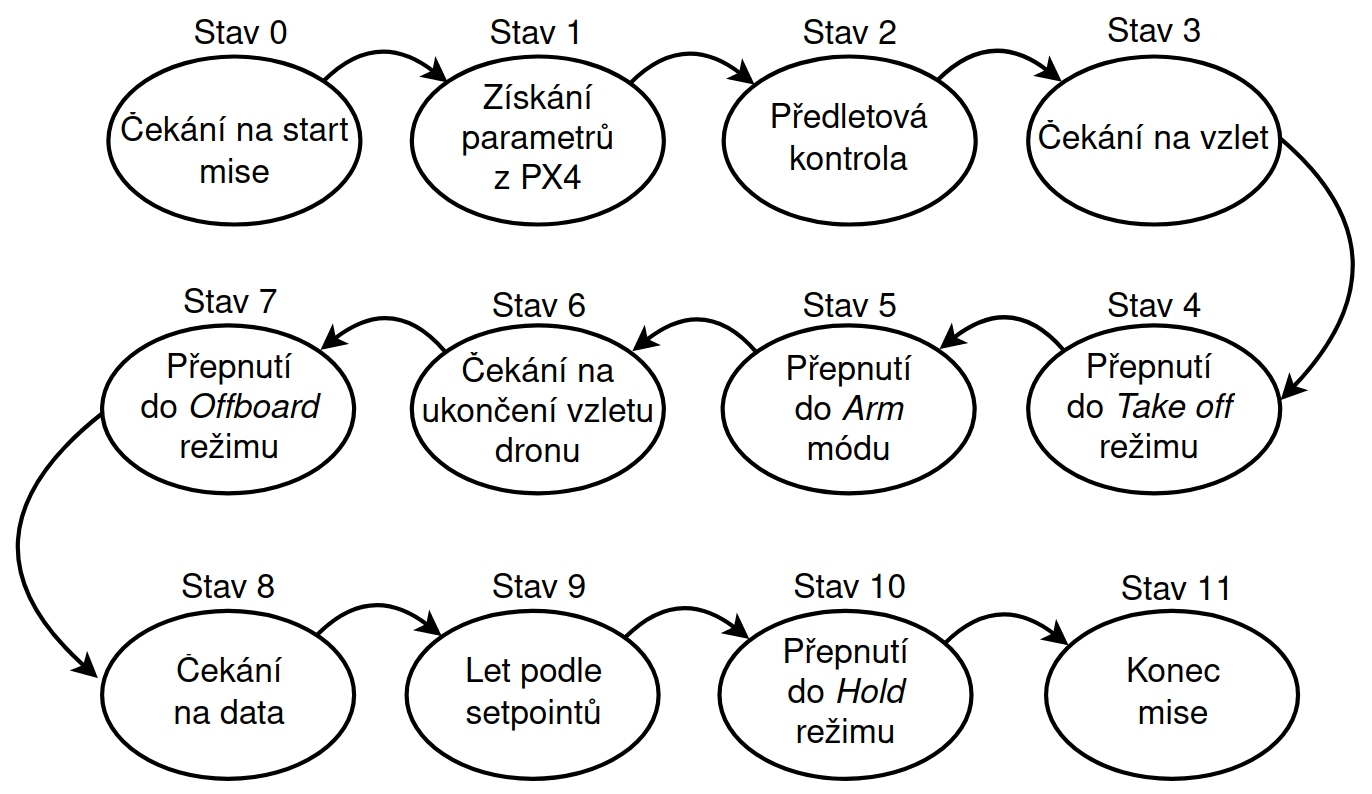
\includegraphics[scale=0.32]{obrazky/MISEAUTOMAT}
  \end{center}
  \caption[Stavový automat řídící robotickou misi]{Stavový automat řídící robotickou misi.}
  \label{fig:MISE2}
\end{figure}

\subsubsection{Stav 0: Čekání na start mise}

Dron je na zemi ve vypnutém stavu.

\noindent\textbf{Podmínka přechodu:} Uběhne uživatelem stanovený čas.

\subsubsection{Stav 1: Získání parametrů z PX4}

Dron vyžádá aktivní parametry ze systému PX4 kvůli tomu, aby bylo možné měnit parametry pomocí komunikačního uzlu Mavros.

\noindent\textbf{Podmínka přechodu:} Komunikační uzel Mavros pošle nadřazenému uzlu, který řídí misi informaci, že systém PX4 poskytl všechny aktivní parametry.

\subsubsection{Stav 2: Předletová kontrola}

V tomto kroku dron vykoná nezbytné kontroly letové způsobilosti jako je kontrola korektní geolokace (GPS \textit{fix}) a nastaví důležité parametry robotické mise jako je výška vzletu, horizontální rychlost, povolení \textit{offboard módu} a chování dronu po výpadku \textit{offboard} módu.

\noindent\textbf{Podmínka přechodu:} Systém PX4 odešle informaci, že všechny parametry byly změněny správně a GPS na dronu je aktivní.

\subsubsection{Stav 3: Čekání na vzlet}

Dron je na zemi ve vypnutém stavu.

\noindent\textbf{Podmínka přechodu:} Uběhne uživatelem stanovený čas.

\subsubsection{Stav 4: Přepnutí dronu do \textit{take off} letového režimu}

Nadřazený systém pošle požadavek pro změnu letového režimu na \textit{take off} letový režim.

\noindent\textbf{Podmínka přechodu:} Systém PX4 pošle odpověď, že letový režim dronu byl úspěšně změněný.

\subsubsection{Stav 5: Přepnutí dronu do \textit{arm} módu}

Nadřazený systém pošle požadavek pro změnu letového režimu.

\noindent\textbf{Podmínka přechodu:} Systém PX4 pošle odpověď, že mód dronu byl úspěšně změněný na \textit{arm}.

\subsubsection{Stav 6: Čekání na ukončení vzletu dronu}

Dron vykonává sekvenci úkonů pro vzlet.

\noindent\textbf{Podmínka přechodu:} Nadřazený systém detekuje změnu letového režimu na \textit{hold} letový režim z důvodu ukončení vzletu.

\subsubsection{Stav 7: Přepnutí dronu do \textit{offboard} letového režimu}

Nadřazený systém pošle požadavek pro změnu letového režimu na \textit{offboard} letový režim.

\noindent\textbf{Podmínka přechodu:} Systém PX4 pošle odpověď, že letový režim dronu byl úspěšně změněný.

\subsubsection{Stav 8: Čekání na data}

Dron se vznáší v \textit{offboard} letovém režimu na místě, kde byla ukončená vzletová sekvence. Tento stav je aktivní jenom v misích, kde jsou data pro let dronu generována a vysílána jiným ROS 2 uzlem, například v misi pro sledování dynamického objektu.

\noindent\textbf{Podmínka přechodu:} ROS 2 uzel pro řízení mise přijme první paket dat.

\subsubsection{Stav 9: Let podle setpointů}

Dron v \textit{offboard} letovém režimu vykonává jednotlivé úkony robotické mise. Nadřazený ROS 2 uzel pro řízení mise posílá dronu buď poziční waypointy (lokální nebo globální), nebo řídí přímo lineární rychlosti v osách \textit{X}, \textit{Y}, \textit{Z} a rychlost rotace kolem osy \textit{Z}.

\noindent\textbf{Podmínka přechodu:} Nadřazený uzel pro řízení mise již nepřímá data pro let dronu (po určitou dobu definovanou uživatelem) nebo dron vykoná všechny úkony robotické mise.

\subsubsection{Stav 10: Přepnutí do \textit{hold} režimu}

Dron se v tomto stavu vznáší v \textit{offboard} letovém režimu na místě, kde ukončil poslední úkon robotické mise. V této fázi je nutný zásah pilota kvůli tomu, že nechceme, aby dron zahájil přistávací manévr bez vědomí a povolení pilota.

\noindent\textbf{Podmínka přechodu:} Pilot dronu převezme řízení dronu.

\subsubsection{Stav 11: Konec mise}

Pilot dronu přistává nebo zahajuje další autonomní misi.

